\documentclass{standalone}
\usepackage{tikz}
\usetikzlibrary{patterns, positioning}


\begin{document}
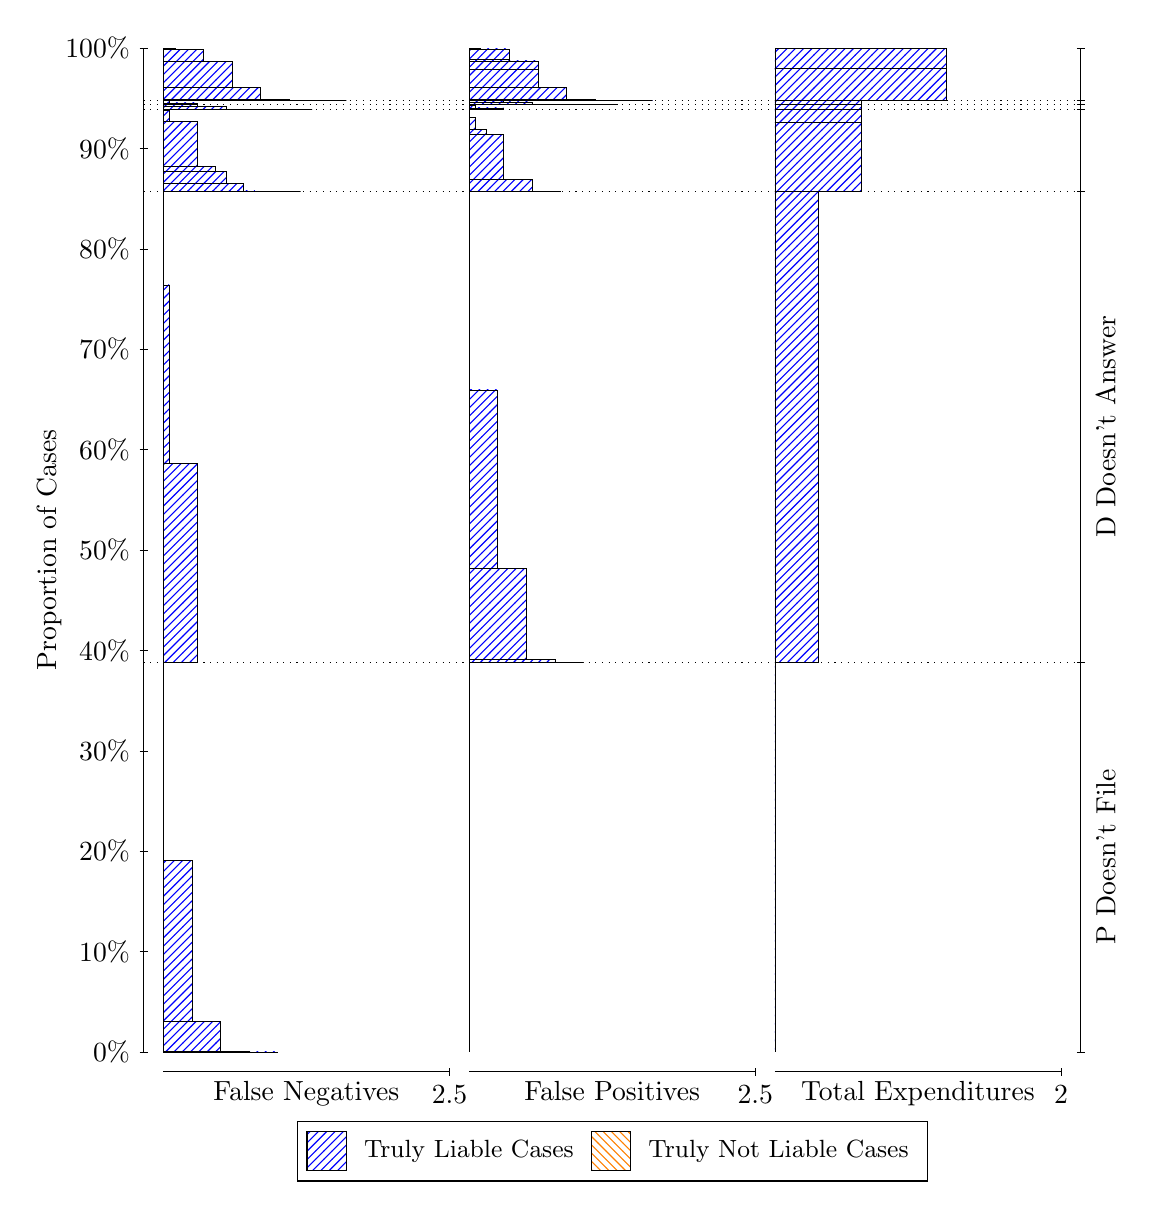
\begin{tikzpicture}
\draw[black, very thin] (1.5,1.75) -- (1.5,14.5);
\node[rotate=90, text=black, anchor=center] at (0.3, 8.125) {Proportion of Cases};
\draw[black, very thin] (1.45,1.75) -- (1.55,1.75);
\node[text=black, anchor=east] at (1.45, 1.75) {0\%};
\draw[black, very thin] (1.45,3.025) -- (1.55,3.025);
\node[text=black, anchor=east] at (1.45, 3.025) {10\%};
\draw[black, very thin] (1.45,4.3) -- (1.55,4.3);
\node[text=black, anchor=east] at (1.45, 4.3) {20\%};
\draw[black, very thin] (1.45,5.575) -- (1.55,5.575);
\node[text=black, anchor=east] at (1.45, 5.575) {30\%};
\draw[black, very thin] (1.45,6.85) -- (1.55,6.85);
\node[text=black, anchor=east] at (1.45, 6.85) {40\%};
\draw[black, very thin] (1.45,8.125) -- (1.55,8.125);
\node[text=black, anchor=east] at (1.45, 8.125) {50\%};
\draw[black, very thin] (1.45,9.4) -- (1.55,9.4);
\node[text=black, anchor=east] at (1.45, 9.4) {60\%};
\draw[black, very thin] (1.45,10.675) -- (1.55,10.675);
\node[text=black, anchor=east] at (1.45, 10.675) {70\%};
\draw[black, very thin] (1.45,11.95) -- (1.55,11.95);
\node[text=black, anchor=east] at (1.45, 11.95) {80\%};
\draw[black, very thin] (1.45,13.225) -- (1.55,13.225);
\node[text=black, anchor=east] at (1.45, 13.225) {90\%};
\draw[black, very thin] (1.45,14.5) -- (1.55,14.5);
\node[text=black, anchor=east] at (1.45, 14.5) {100\%};

\draw[black, very thin] (13.4,1.75) -- (13.4,14.5);
\draw[black, very thin] (13.35,1.75) -- (13.45,1.75);
\node[anchor=west] at (13.35, 1.75) {};
\draw[black, very thin] (13.35,6.7003) -- (13.45,6.7003);
\node[anchor=west] at (13.35, 6.7003) {};
\draw[black, very thin] (13.35,12.681) -- (13.45,12.681);
\node[anchor=west] at (13.35, 12.681) {};
\draw[black, very thin] (13.35,13.718) -- (13.45,13.718);
\node[anchor=west] at (13.35, 13.718) {};
\draw[black, very thin] (13.35,13.781) -- (13.45,13.781);
\node[anchor=west] at (13.35, 13.781) {};
\draw[black, very thin] (13.35,13.838) -- (13.45,13.838);
\node[anchor=west] at (13.35, 13.838) {};
\draw[black, very thin] (13.35,14.5) -- (13.45,14.5);
\node[anchor=west] at (13.35, 14.5) {};

\draw[black, very thin, pattern color=blue, pattern=north east lines] (1.75,1.75) rectangle (3.2033,1.75);
\draw[black, very thin, pattern color=blue, pattern=north east lines] (1.75,1.75) rectangle (2.84,1.7532);
\draw[black, very thin, pattern color=blue, pattern=north east lines] (1.75,1.7532) rectangle (2.4767,2.1351);
\draw[black, very thin, pattern color=blue, pattern=north east lines] (1.75,2.1351) rectangle (2.1133,4.1813);
\draw[black, very thin, pattern color=orange, pattern=north west lines] (1.75,4.1813) rectangle (1.75,4.1813);
\draw[black, very thin, pattern color=blue, pattern=north east lines] (1.75,4.1813) rectangle (1.75,6.7003);
\draw[black, very thin, pattern color=blue, pattern=north east lines] (1.75,6.7003) rectangle (2.186,9.2217);
\draw[black, very thin, pattern color=blue, pattern=north east lines] (1.75,9.2217) rectangle (1.8227,11.493);
\draw[black, very thin, pattern color=orange, pattern=north west lines] (1.75,11.493) rectangle (1.75,11.493);
\draw[black, very thin, pattern color=blue, pattern=north east lines] (1.75,11.493) rectangle (1.75,12.681);
\draw[black, very thin, pattern color=blue, pattern=north east lines] (1.75,12.681) rectangle (3.494,12.681);
\draw[black, very thin, pattern color=blue, pattern=north east lines] (1.75,12.681) rectangle (3.1307,12.683);
\draw[black, very thin, pattern color=blue, pattern=north east lines] (1.75,12.683) rectangle (2.9127,12.687);
\draw[black, very thin, pattern color=blue, pattern=north east lines] (1.75,12.687) rectangle (2.7673,12.778);
\draw[black, very thin, pattern color=blue, pattern=north east lines] (1.75,12.778) rectangle (2.5493,12.93);
\draw[black, very thin, pattern color=blue, pattern=north east lines] (1.75,12.93) rectangle (2.404,13);
\draw[black, very thin, pattern color=blue, pattern=north east lines] (1.75,13) rectangle (2.186,13.57);
\draw[black, very thin, pattern color=blue, pattern=north east lines] (1.75,13.57) rectangle (2.0407,13.571);
\draw[black, very thin, pattern color=blue, pattern=north east lines] (1.75,13.571) rectangle (1.8227,13.714);
\draw[black, very thin, pattern color=orange, pattern=north west lines] (1.75,13.714) rectangle (1.75,13.714);
\draw[black, very thin, pattern color=blue, pattern=north east lines] (1.75,13.714) rectangle (1.75,13.718);
\draw[black, very thin, pattern color=blue, pattern=north east lines] (1.75,13.718) rectangle (3.6393,13.718);
\draw[black, very thin, pattern color=blue, pattern=north east lines] (1.75,13.718) rectangle (3.276,13.718);
\draw[black, very thin, pattern color=blue, pattern=north east lines] (1.75,13.718) rectangle (2.9127,13.719);
\draw[black, very thin, pattern color=blue, pattern=north east lines] (1.75,13.719) rectangle (2.5493,13.757);
\draw[black, very thin, pattern color=blue, pattern=north east lines] (1.75,13.757) rectangle (2.186,13.781);
\draw[black, very thin, pattern color=orange, pattern=north west lines] (1.75,13.781) rectangle (1.75,13.781);
\draw[black, very thin, pattern color=blue, pattern=north east lines] (1.75,13.781) rectangle (2.186,13.804);
\draw[black, very thin, pattern color=blue, pattern=north east lines] (1.75,13.804) rectangle (1.8227,13.837);
\draw[black, very thin, pattern color=orange, pattern=north west lines] (1.75,13.837) rectangle (1.75,13.837);
\draw[black, very thin, pattern color=blue, pattern=north east lines] (1.75,13.837) rectangle (1.75,13.838);
\draw[black, very thin, pattern color=blue, pattern=north east lines] (1.75,13.838) rectangle (4.0753,13.838);
\draw[black, very thin, pattern color=blue, pattern=north east lines] (1.75,13.838) rectangle (3.712,13.838);
\draw[black, very thin, pattern color=blue, pattern=north east lines] (1.75,13.838) rectangle (3.3487,13.848);
\draw[black, very thin, pattern color=blue, pattern=north east lines] (1.75,13.848) rectangle (2.9853,14.001);
\draw[black, very thin, pattern color=blue, pattern=north east lines] (1.75,14.001) rectangle (2.622,14.333);
\draw[black, very thin, pattern color=blue, pattern=north east lines] (1.75,14.333) rectangle (2.2587,14.487);
\draw[black, very thin, pattern color=blue, pattern=north east lines] (1.75,14.487) rectangle (1.8953,14.5);
\draw[black, very thin, pattern color=orange, pattern=north west lines] (1.75,14.5) rectangle (1.75,14.5);
\draw[black, very thin, pattern color=blue, pattern=north east lines] (1.75,14.5) rectangle (1.75,14.5);
\draw[black, very thin, pattern color=orange, pattern=north west lines] (5.6333,1.75) rectangle (5.6333,1.75);
\draw[black, very thin, pattern color=blue, pattern=north east lines] (5.6333,1.75) rectangle (5.6333,6.7003);
\draw[black, very thin, pattern color=orange, pattern=north west lines] (5.6333,6.7003) rectangle (7.0867,6.7003);
\draw[black, very thin, pattern color=blue, pattern=north east lines] (5.6333,6.7003) rectangle (7.0867,6.7003);
\draw[black, very thin, pattern color=blue, pattern=north east lines] (5.6333,6.7003) rectangle (6.7233,6.7369);
\draw[black, very thin, pattern color=blue, pattern=north east lines] (5.6333,6.7369) rectangle (6.36,7.8881);
\draw[black, very thin, pattern color=blue, pattern=north east lines] (5.6333,7.8881) rectangle (5.9967,10.159);
\draw[black, very thin, pattern color=blue, pattern=north east lines] (5.6333,10.159) rectangle (5.6333,12.681);
\draw[black, very thin, pattern color=orange, pattern=north west lines] (5.6333,12.681) rectangle (6.796,12.681);
\draw[black, very thin, pattern color=blue, pattern=north east lines] (5.6333,12.681) rectangle (6.796,12.684);
\draw[black, very thin, pattern color=blue, pattern=north east lines] (5.6333,12.684) rectangle (6.4327,12.828);
\draw[black, very thin, pattern color=orange, pattern=north west lines] (5.6333,12.828) rectangle (6.2147,12.828);
\draw[black, very thin, pattern color=blue, pattern=north east lines] (5.6333,12.828) rectangle (6.2147,12.829);
\draw[black, very thin, pattern color=blue, pattern=north east lines] (5.6333,12.829) rectangle (6.0693,13.399);
\draw[black, very thin, pattern color=blue, pattern=north east lines] (5.6333,13.399) rectangle (5.8513,13.468);
\draw[black, very thin, pattern color=blue, pattern=north east lines] (5.6333,13.468) rectangle (5.706,13.621);
\draw[black, very thin, pattern color=blue, pattern=north east lines] (5.6333,13.621) rectangle (5.6333,13.718);
\draw[black, very thin, pattern color=orange, pattern=north west lines] (5.6333,13.718) rectangle (6.0693,13.718);
\draw[black, very thin, pattern color=blue, pattern=north east lines] (5.6333,13.718) rectangle (6.0693,13.741);
\draw[black, very thin, pattern color=blue, pattern=north east lines] (5.6333,13.741) rectangle (5.706,13.779);
\draw[black, very thin, pattern color=blue, pattern=north east lines] (5.6333,13.779) rectangle (5.6333,13.781);
\draw[black, very thin, pattern color=orange, pattern=north west lines] (5.6333,13.781) rectangle (7.5227,13.781);
\draw[black, very thin, pattern color=blue, pattern=north east lines] (5.6333,13.781) rectangle (7.5227,13.781);
\draw[black, very thin, pattern color=blue, pattern=north east lines] (5.6333,13.781) rectangle (7.1593,13.781);
\draw[black, very thin, pattern color=blue, pattern=north east lines] (5.6333,13.781) rectangle (6.796,13.782);
\draw[black, very thin, pattern color=blue, pattern=north east lines] (5.6333,13.782) rectangle (6.4327,13.815);
\draw[black, very thin, pattern color=blue, pattern=north east lines] (5.6333,13.815) rectangle (6.0693,13.838);
\draw[black, very thin, pattern color=orange, pattern=north west lines] (5.6333,13.838) rectangle (7.9587,13.838);
\draw[black, very thin, pattern color=blue, pattern=north east lines] (5.6333,13.838) rectangle (7.9587,13.838);
\draw[black, very thin, pattern color=orange, pattern=north west lines] (5.6333,13.838) rectangle (7.5953,13.838);
\draw[black, very thin, pattern color=blue, pattern=north east lines] (5.6333,13.838) rectangle (7.5953,13.838);
\draw[black, very thin, pattern color=orange, pattern=north west lines] (5.6333,13.838) rectangle (7.232,13.838);
\draw[black, very thin, pattern color=blue, pattern=north east lines] (5.6333,13.838) rectangle (7.232,13.851);
\draw[black, very thin, pattern color=blue, pattern=north east lines] (5.6333,13.851) rectangle (6.8687,14.004);
\draw[black, very thin, pattern color=orange, pattern=north west lines] (5.6333,14.004) rectangle (6.8687,14.004);
\draw[black, very thin, pattern color=blue, pattern=north east lines] (5.6333,14.004) rectangle (6.8687,14.005);
\draw[black, very thin, pattern color=blue, pattern=north east lines] (5.6333,14.005) rectangle (6.5053,14.225);
\draw[black, very thin, pattern color=orange, pattern=north west lines] (5.6333,14.225) rectangle (6.5053,14.225);
\draw[black, very thin, pattern color=blue, pattern=north east lines] (5.6333,14.225) rectangle (6.5053,14.337);
\draw[black, very thin, pattern color=blue, pattern=north east lines] (5.6333,14.337) rectangle (6.142,14.358);
\draw[black, very thin, pattern color=blue, pattern=north east lines] (5.6333,14.358) rectangle (6.142,14.49);
\draw[black, very thin, pattern color=blue, pattern=north east lines] (5.6333,14.49) rectangle (5.7787,14.49);
\draw[black, very thin, pattern color=blue, pattern=north east lines] (5.6333,14.49) rectangle (5.7787,14.5);
\draw[black, very thin, pattern color=blue, pattern=north east lines] (5.6333,14.5) rectangle (5.6333,14.5);
\draw[black, very thin, pattern color=orange, pattern=north west lines] (9.5167,1.75) rectangle (9.5167,1.75);
\draw[black, very thin, pattern color=blue, pattern=north east lines] (9.5167,1.75) rectangle (9.5167,6.7003);
\draw[black, very thin, pattern color=orange, pattern=north west lines] (9.5167,6.7003) rectangle (10.062,6.7003);
\draw[black, very thin, pattern color=blue, pattern=north east lines] (9.5167,6.7003) rectangle (10.062,12.681);
\draw[black, very thin, pattern color=orange, pattern=north west lines] (9.5167,12.681) rectangle (10.607,12.681);
\draw[black, very thin, pattern color=blue, pattern=north east lines] (9.5167,12.681) rectangle (10.607,13.554);
\draw[black, very thin, pattern color=orange, pattern=north west lines] (9.5167,13.554) rectangle (10.607,13.554);
\draw[black, very thin, pattern color=blue, pattern=north east lines] (9.5167,13.554) rectangle (10.607,13.718);
\draw[black, very thin, pattern color=orange, pattern=north west lines] (9.5167,13.718) rectangle (10.607,13.718);
\draw[black, very thin, pattern color=blue, pattern=north east lines] (9.5167,13.718) rectangle (10.607,13.781);
\draw[black, very thin, pattern color=orange, pattern=north west lines] (9.5167,13.781) rectangle (10.607,13.781);
\draw[black, very thin, pattern color=blue, pattern=north east lines] (9.5167,13.781) rectangle (10.607,13.838);
\draw[black, very thin, pattern color=orange, pattern=north west lines] (9.5167,13.838) rectangle (11.697,13.838);
\draw[black, very thin, pattern color=blue, pattern=north east lines] (9.5167,13.838) rectangle (11.697,14.245);
\draw[black, very thin, pattern color=orange, pattern=north west lines] (9.5167,14.245) rectangle (11.697,14.245);
\draw[black, very thin, pattern color=blue, pattern=north east lines] (9.5167,14.245) rectangle (11.697,14.5);
\draw[black, dotted] (1.5,6.7003) -- (13.4,6.7003);
\draw[black, dotted] (1.5,12.681) -- (13.4,12.681);
\draw[black, dotted] (1.5,13.718) -- (13.4,13.718);
\draw[black, dotted] (1.5,13.781) -- (13.4,13.781);
\draw[black, dotted] (1.5,13.838) -- (13.4,13.838);
\draw[black, very thin] (1.75,1.5) -- (5.3833,1.5);
\node[text=black, anchor=north] at (3.5667, 1.5) {False Negatives};
\draw[black, very thin] (5.3833,1.45) -- (5.3833,1.55);
\node[text=black, anchor=north] at (5.3833, 1.45) {2.5};

\draw[black, very thin] (5.6333,1.5) -- (9.2667,1.5);
\node[text=black, anchor=north] at (7.45, 1.5) {False Positives};
\draw[black, very thin] (9.2667,1.45) -- (9.2667,1.55);
\node[text=black, anchor=north] at (9.2667, 1.45) {2.5};

\draw[black, very thin] (9.5167,1.5) -- (13.15,1.5);
\node[text=black, anchor=north] at (11.333, 1.5) {Total Expenditures};
\draw[black, very thin] (13.15,1.45) -- (13.15,1.55);
\node[text=black, anchor=north] at (13.15, 1.45) {2};

\node[text=black, centered, rotate=90] at (13.72, 4.2251) {P Doesn't File};
\node[text=black, centered, rotate=90] at (13.72, 9.6904) {D Doesn't Answer};





\draw (7.449999999999999,1.5) node[draw=none] (baseCoordinate) {};
\begin{scope}[align=center]
        \matrix[scale=0.5, draw=black, below=0.5cm of baseCoordinate, nodes={draw}, column sep=0.1cm]{
            \node[rectangle, draw, minimum width=0.5cm, minimum height=0.5cm, pattern color=blue, pattern=north east lines] {}; &
            \node[draw=none, font=\small, text=black] (B) {Truly Liable Cases}; &
            \node[rectangle, draw, minimum width=0.5cm, minimum height=0.5cm, pattern color=orange, pattern=north west lines] {}; &
            \node[draw=none, font=\small, text=black] (B) {Truly Not Liable Cases}; \\
            };
\end{scope}

\end{tikzpicture}
\end{document}